% Enable warnings about problematic code
\RequirePackage[l2tabu, orthodox]{nag}

\documentclass{resources/WeSTassignment}
\usepackage{tabularx}
\usepackage{booktabs}
\usepackage[utf8]{inputenc}
\usepackage{amsmath}
\usepackage{graphics}
\usepackage{graphicx}
\usepackage{changebar}
\usepackage{latexsym}
\usepackage{stmaryrd}
\usepackage{booktabs}
\usepackage{amsmath}
\usepackage{wasysym}
\usepackage[export]{adjustbox}
\usepackage[thinlines]{easytable}
\usepackage{framed}
\usepackage{color}
\usepackage{footnote}
\usepackage{listings}
\usepackage{framed}
\usepackage{url}
\usepackage[T1]{fontenc}
\usepackage{lmodern}

% The lecture title, e.g. "Web Information Retrieval".
\lecture{Introduction to Web Science}
% The names of the lecturer and the instructor(s)
\author{%
  PD Dr. Matthias~Thimm\\{\normalsize\mailto{thimm@uni-koblenz.de}} \and
  Ipek~Baris Schlicht\\{\normalsize\mailto{ibaris@uni-koblenz.de}} \and
  Kenneth Skiba\\{\normalsize\mailto{kennethskiba@uni-koblenz.de}}
}
% Assignment number.
\assignmentnumber{5}
% Institute of lecture.
\institute{%
  Institute of Web Science and Technologies\\%
  Department of Computer Science\\%
  University of Koblenz-Landau%
}
% Date until students should submit their solutions.
\datesubmission{15.12.2020, CEST 23:59}

% Specify bib file location.
\addbibresource{bibliography.bib}

\begin{document}

\maketitle

\centering \textbf{Team:} Bravo\\
\centering \textbf{Members:}\\
\centering  Gaurav Kumar (220200656)\\
\centering  Pavithree Shetty (220200661)\\
\centering  Nisha Sharma (220202359)\\

\section{Analysis of Simple English Wikipedia\hfill{60 Points}}
\subsection{Crawling}
Your task in this exercise is to crawl the Simple English Wikipedia. In order to execute this task, please first follow the steps in \textbf{Installation}.

\textbf{Installation} \\

In order to solve the task, you are required to download Simple English Wiki Dump \texttt{wikipedia\_en\_simple\_all\_nopic\_2020-10.zim} and then set up \texttt{dockerized} \texttt{Kiwix Server} for hosting the Wiki locally. Please follow these installation steps:
\begin{enumerate}
    \item Install a \texttt{Docker} engine (\url{https://docs.docker.com/engine/install/}) if your computer does not have one. 
    \item Download the Simple English Wiki 2020 (\texttt{wikipedia\_en\_simple\_all\_nopic\_2020-10.zim}) from the website (\url{https://ftp.fau.de/kiwix/zim/wikipedia/}). The size of the file is 481M and it does not contain pictures. 
    \item Clone the repository (\url{https://github.com/isspek/dockerized-kiwix-server})  where you can find the installation scripts for installing Wiki Server using \texttt{Docker}. Follow the installation steps in the repository.
    \item You are supposed to see Simple English Wikipedia at \texttt{localhost:8080}, when the installation is successfully complete.  
\end{enumerate}

\textbf{Task} \\
You can start crawling from \url{http://localhost:8080/wikipedia_en_simple_all_nopic_2020-10/A/COVID-19_pandemic} as seed set and you can use the libraries \textcolor{red}{\texttt{beautifulsoup}}, \textcolor{red}{\texttt{request}, \texttt{urllib}, \texttt{pandas}, \texttt{re}, \texttt{numpy}, \texttt{collections}, \texttt{logging}, \texttt{pickle}, \texttt{sys}, \texttt{dataclasses}, \texttt{matplotlib}}.

A simple crawler has minimum following units:\\
\begin{enumerate}
    \item A fetcher for retrieving urls.
    \item A parser for extracting contents.
    \item A filter to handle duplicate or already fetched urls.
\end{enumerate}
Additionally you are expected to handle any errors such as memory leak, http errors. 

\textbf{Hints} \\

\begin{itemize}
    \item Before you start this exercise, please have a look at \ref{web_crawl_stats}. 
    \item Make really sure your crawler does not follow external urls to domains other than \url{http://localhost:8080/wikipedia_en_simple_all_nopic_2020-10/A/}.
    \item Crawling all pages might take time, be patient.
    \item It might be useful for you to have some output on the crawlers command line depicting, which URL is currently being fetched and how many URLs have been fetched so far and how many are currently on the queue.
    \item  You can (but don’t have to) make use of breadth-first search.
    \item You can (but you don’t have to) speed up the crawler significantly if you use multithreading.
\end{itemize}

\subsection{Limitations} 
Briefly explain the potential limitations of your crawler (max 200 words). \textbf{Hint:} Think use cases for different websites when you use your crawler.
\newline
\newline
\textbf{Solution}
\begin{itemize}
    \item \textbf{Difficult to Analyze:} For anybody, the extracting process is confusing to read. 
    \item \textbf{Data Analysis:} The links that has been extracted will first need to be treated so that they can be easily understood. In some cases, this might take a long time and a lot of energy to complete.
    \item \textbf{Time:} It is normal for new data extraction applications to take some time in the beginning to become familiar with the core application and need to adjust to the scrapping language.
    \item \textbf{Speed and protection policies:} Most web scrapping services are slower than API calls and another problem is the websites that do not allow screen scraping. In such cases, web scrapping services are rendered useless.
\end{itemize}

\subsection{Web Crawl Statistics\label{web_crawl_stats}}

If you have successfully completed the first exercise of this assignment, then please provide the following details:

\begin{enumerate}
\item Total number of links that you fetched in the complete process of crawling.
\item Top 10 Wiki pages that have been linked more than once. Print them with their counts and save them as bar plot figure.
\item Top 10 external pages (pages with a domain which is not \texttt{wikipedia\_en\_simple\_all\_nopic\_2020-10}) that have been linked more than once. Print them with their counts and save them as bar plot figure.
\item For every Wiki page that you have read, count the unique number of internal links and external links. Then provide a histogram for internal links and external links. You can use a bin size of 5 and limit ranges between 0 and 50. Make sure that there is a title indicating mean and sigma values. Save both histogram in separate files.
\item Additionally, save print logs of your task as a file with \texttt{.log} extension.
\end{enumerate}
\begin{figure}[h]
    \centering
    
\includegraphics[scale=0.5]{resources/crawl_count.png}
    \caption{Total Crawl count, only internal}  
    \label{fig:crawl count}
\end{figure}
\begin{figure}[h]
    \centering
    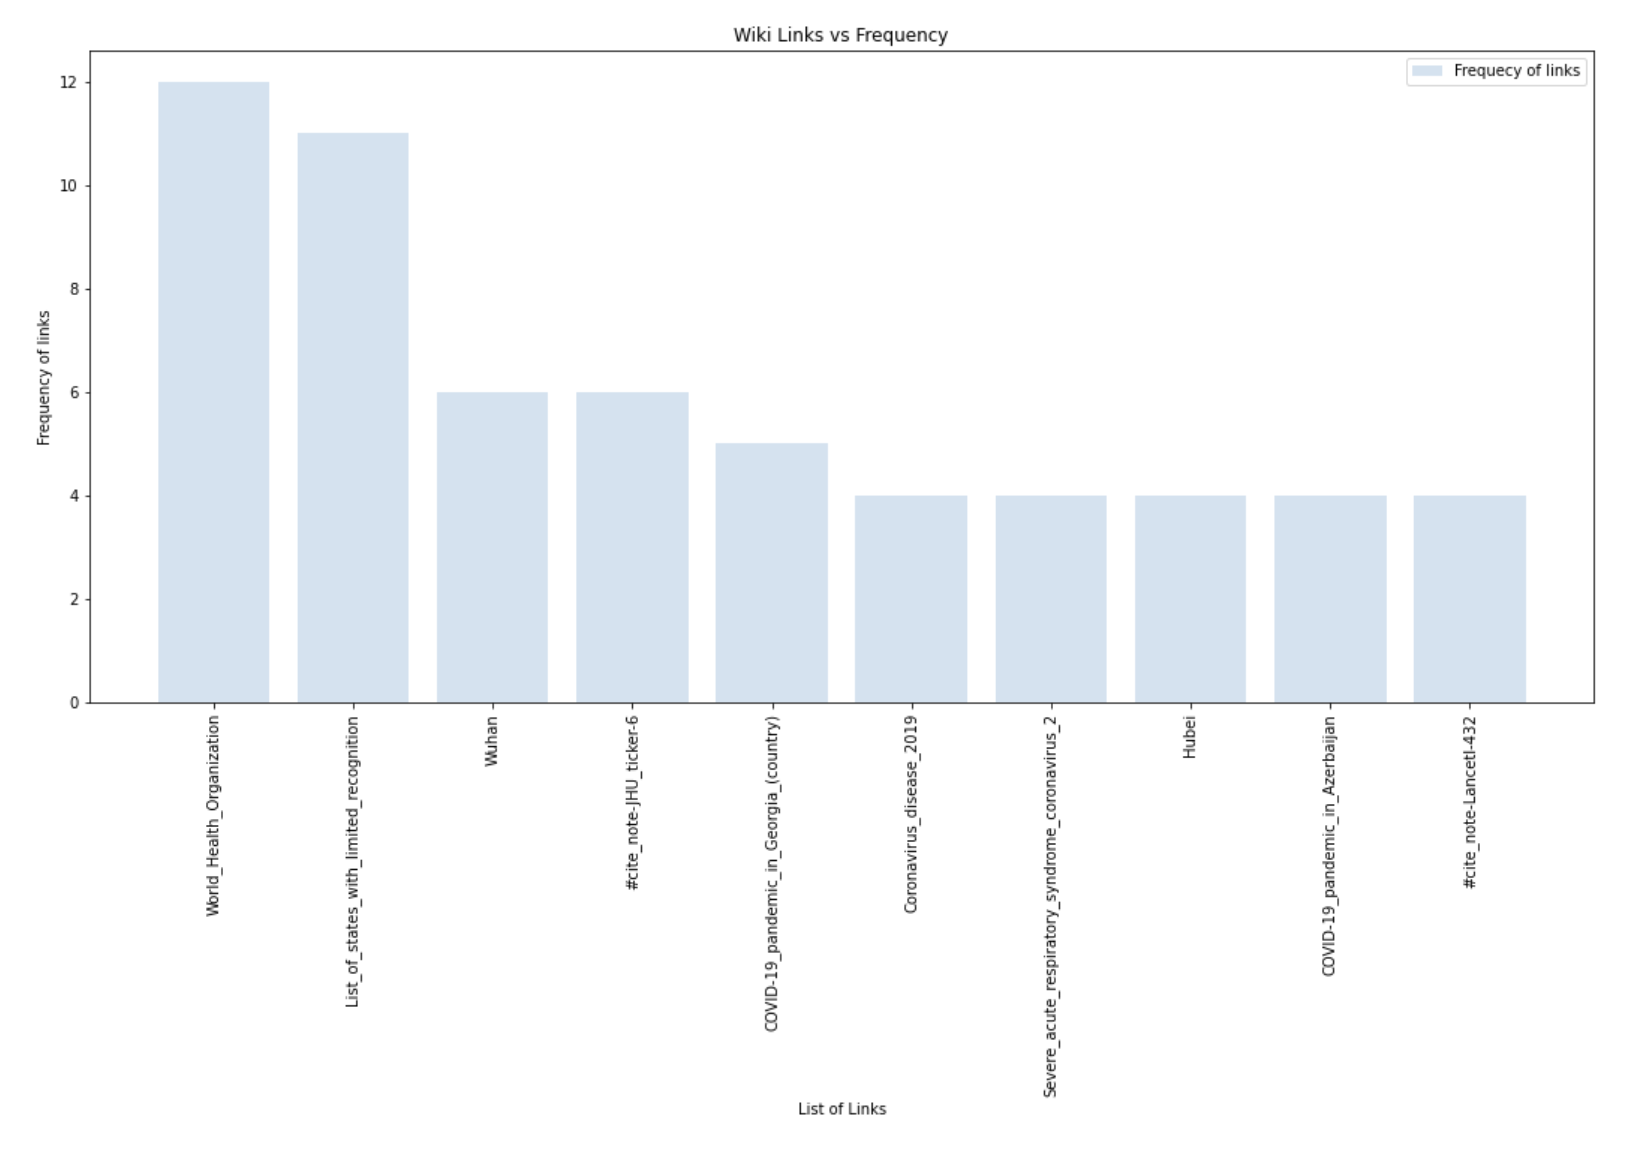
\includegraphics[scale=0.5]{resources/internal.png}
    \caption{Wiki top 10 pages}  
    \label{fig:Wiki top 10 pages}
\end{figure}
\begin{figure}[h]
    \centering
    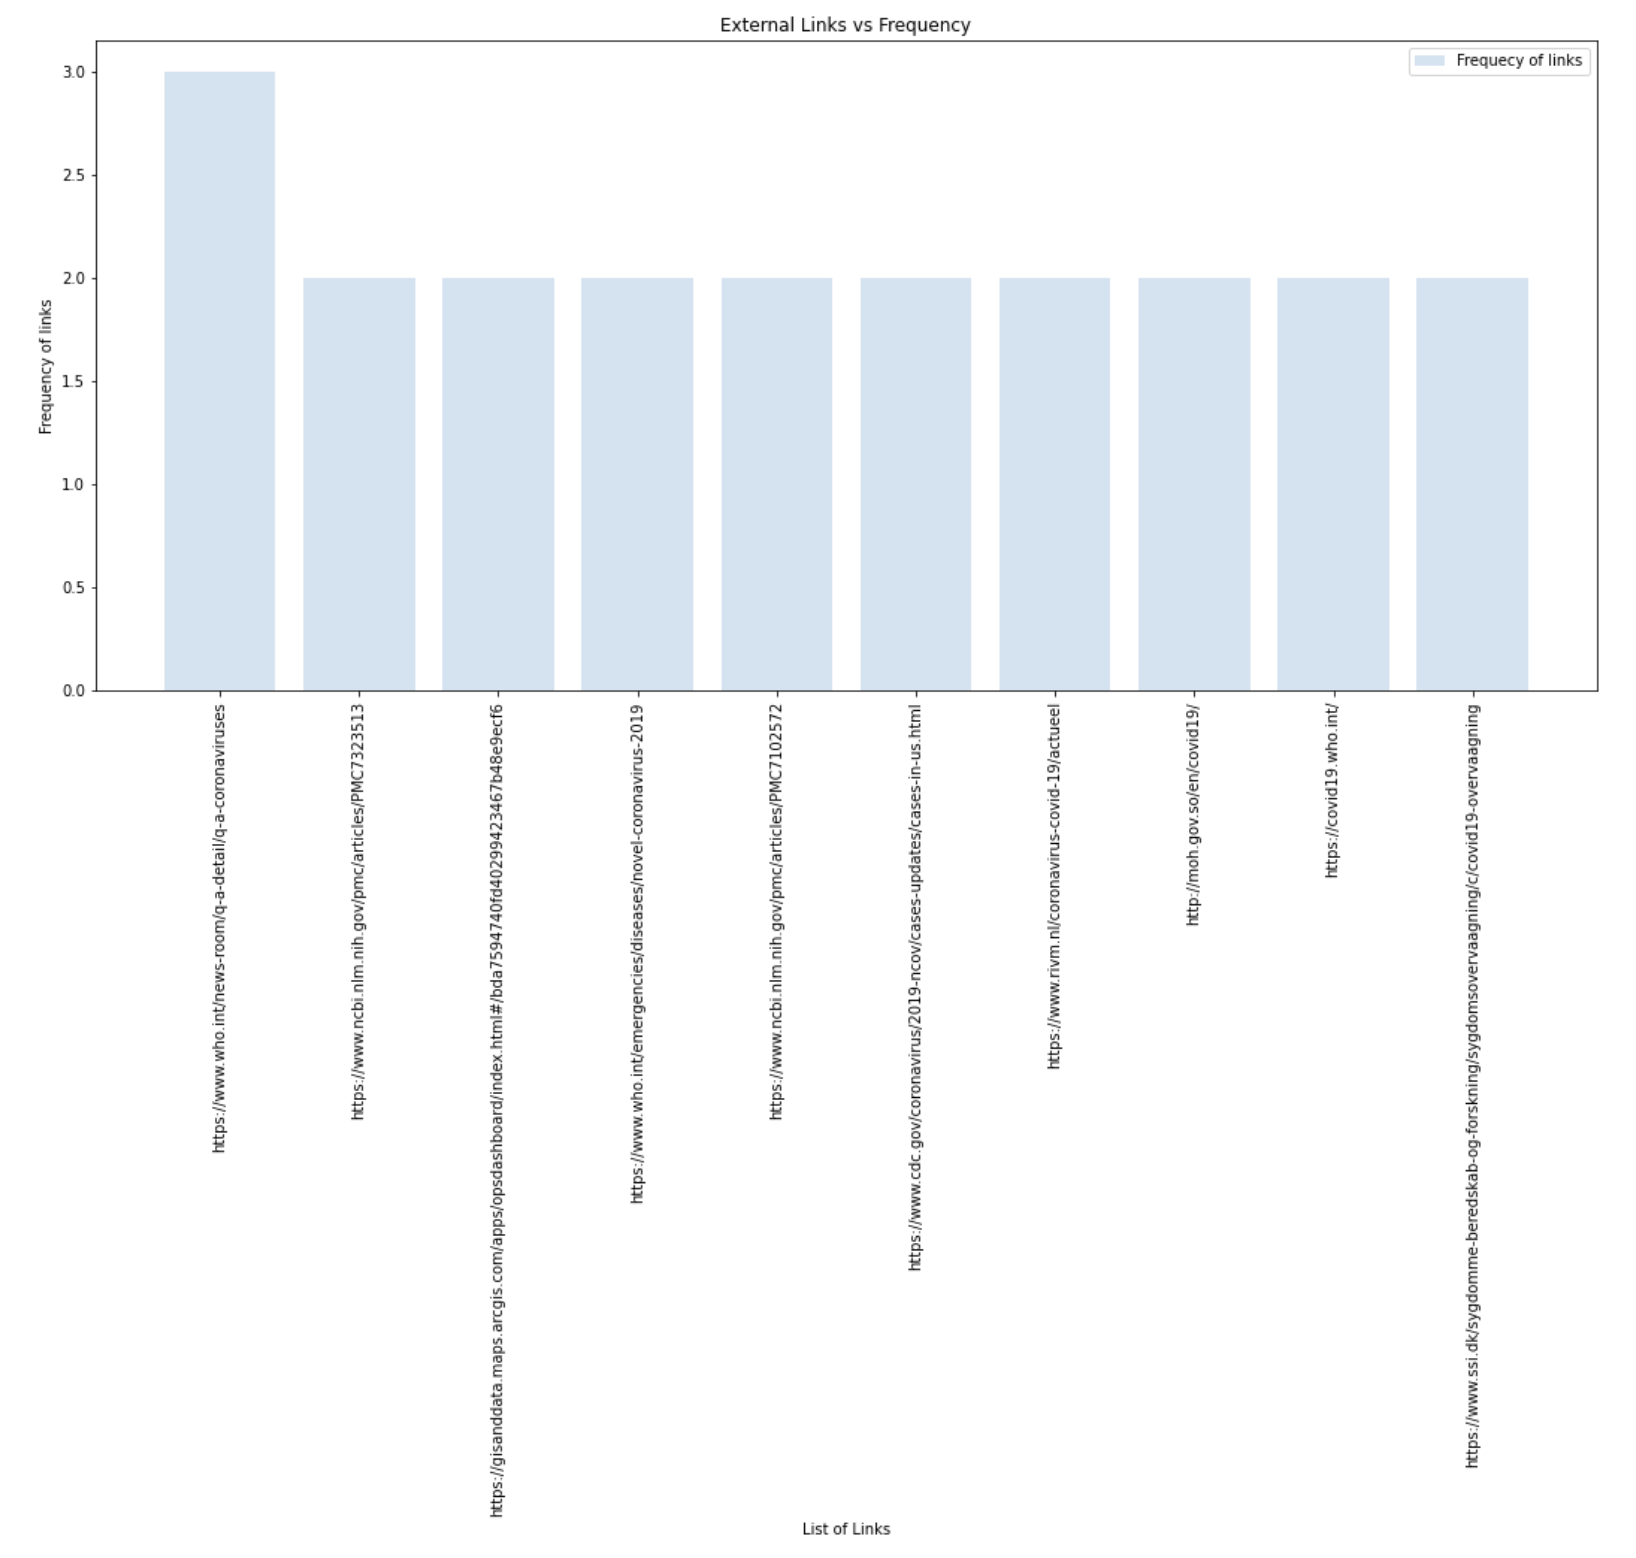
\includegraphics[scale=0.5]{resources/external.png}
    \caption{External top 10 pages}  
    \label{fig:External top 10 pages}
\end{figure}
\begin{figure}[h]
    \centering
    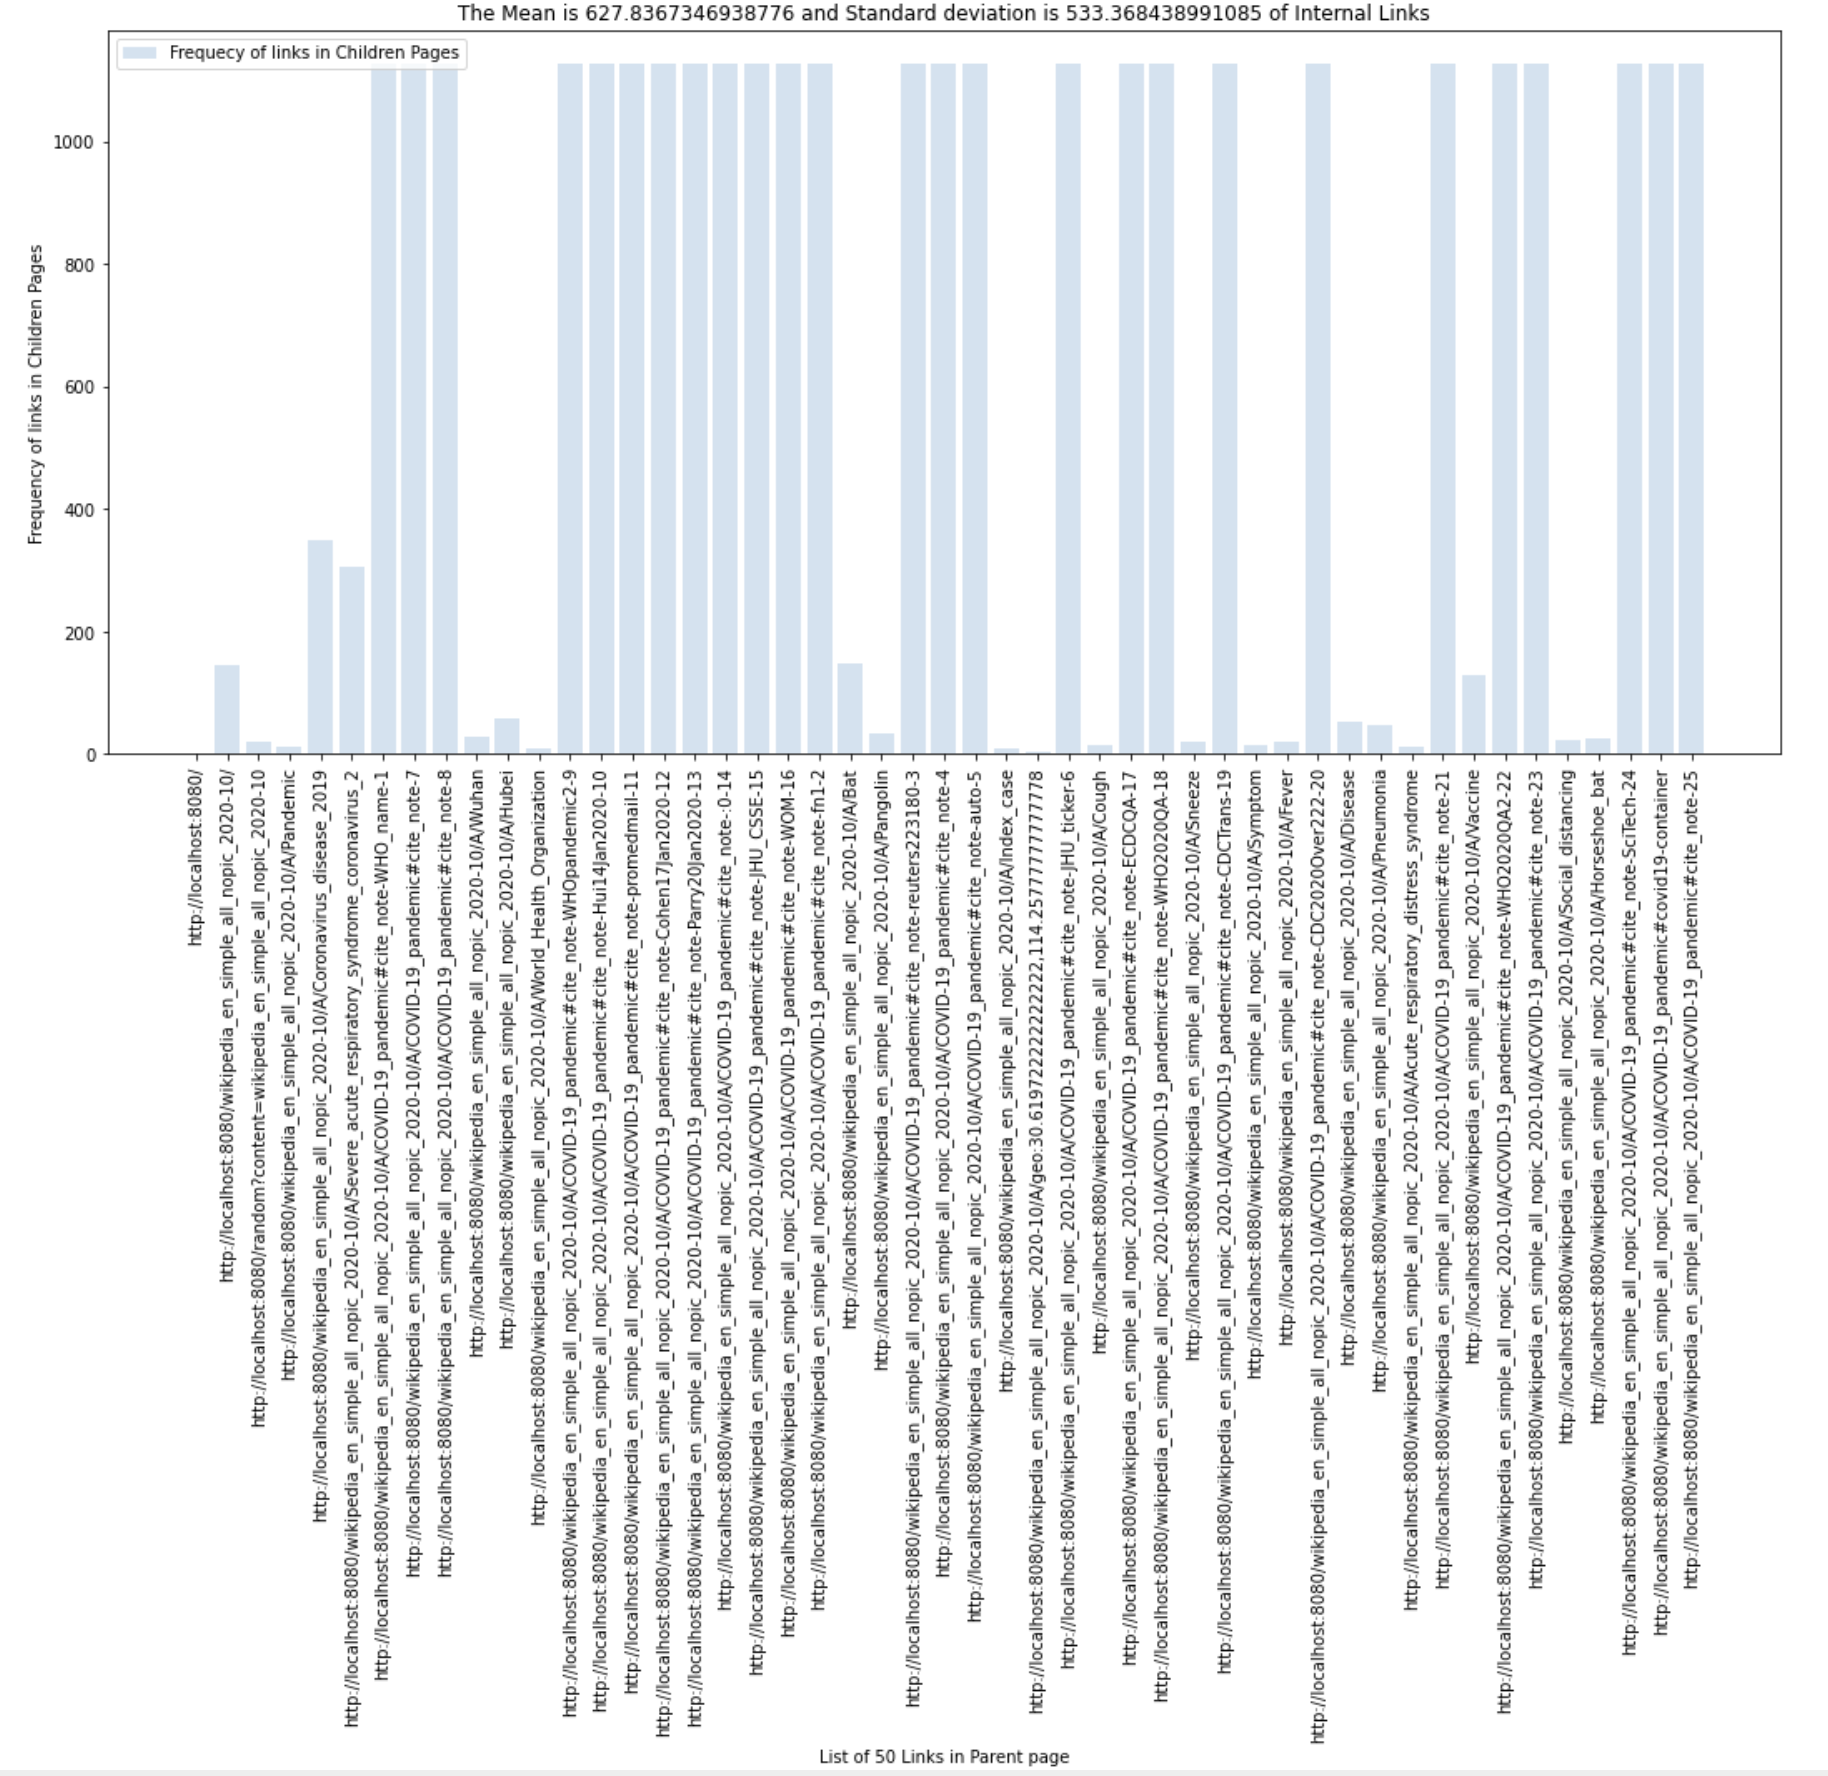
\includegraphics[scale=0.5]{resources/children_internal.png}
    \caption{Mean and Standard deviation of Internal Links}  
    \label{fig:Mean and Standard deviation of Internal Links}
\end{figure}
\begin{figure}[h]
    \centering
    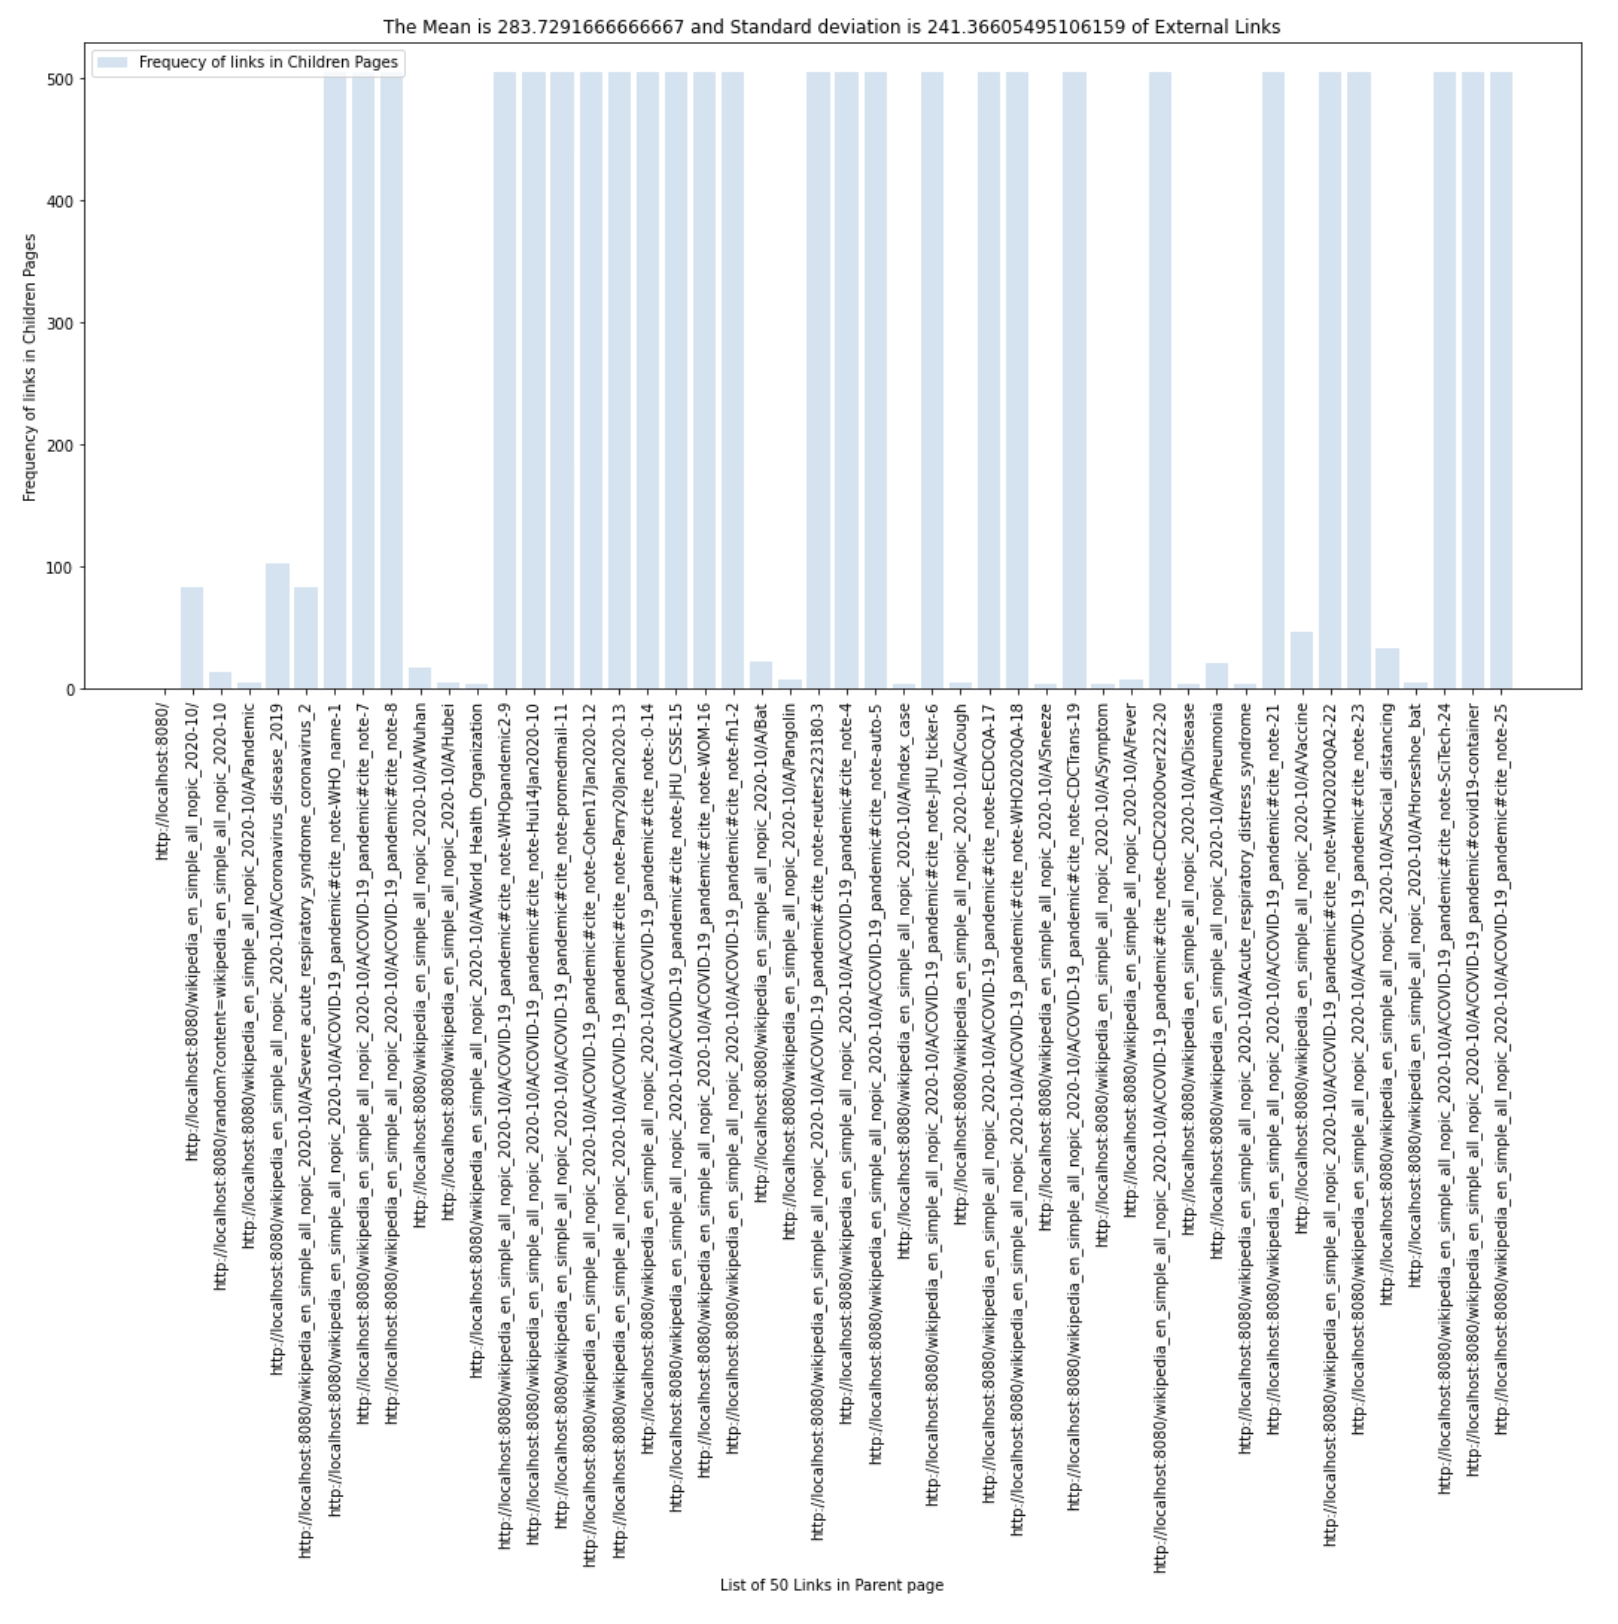
\includegraphics[scale=0.5]{resources/children_external.png}
    \caption{Mean and Standard deviation of External Links}  
    \label{fig:Mean and Standard deviation of External Links}
\end{figure}
\begin{figure}[h]
    \centering
    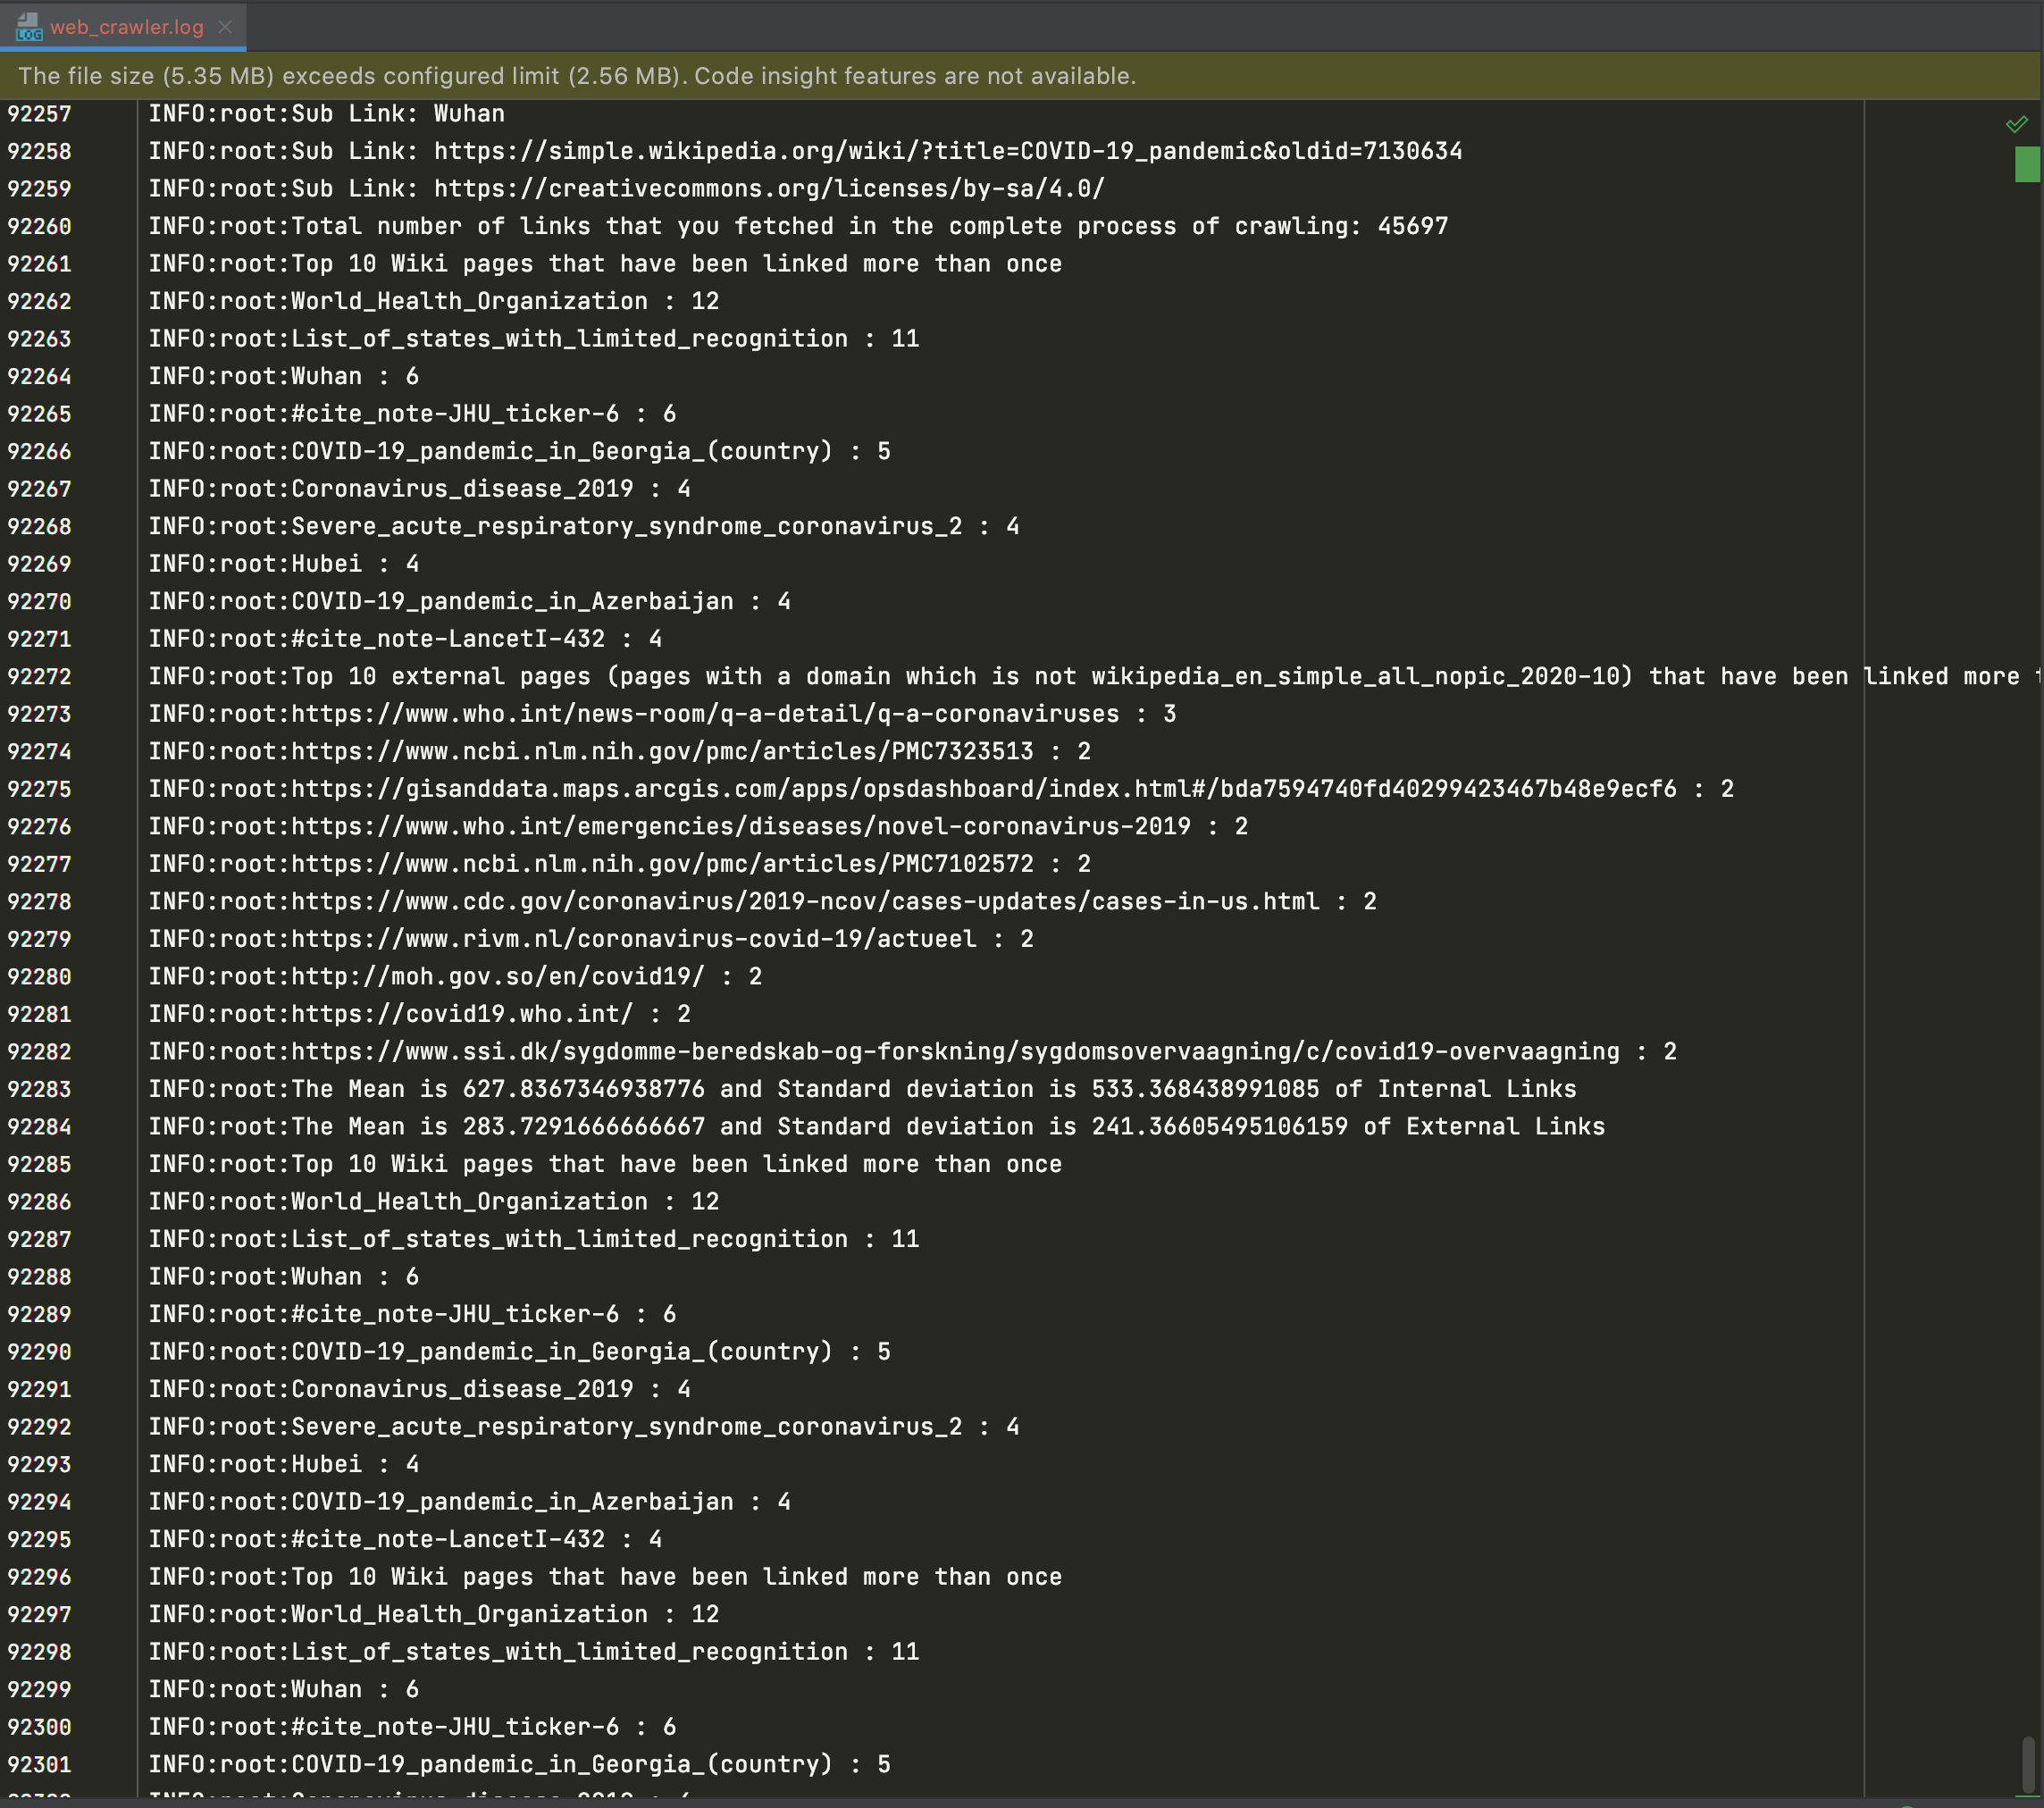
\includegraphics[scale=0.5]{resources/log-file.png}
    \caption{Log file}  
    \label{fig:Log file}
\end{figure}

\section{Questions \hfill{20 Points}}
Answer the following questions with your own words.  
\begin{enumerate}
    \item Why do we have to run probabilistical model more then once? (max 200 words)
    \begin{enumerate}
    \item Random variables and probability distributions are incorporated into the model of an event or phenomenon in probabilistic models, giving a probability distribution as a solution.
    \item Since Probabilistic models involve random process, we will not get the exact same results everytime we run the model.
	\item By running it just once it can produce possible outliers.
	\item So we run the probabilistic model several times to get the most optimum result.
	\item Also,By running it more than once we get statistical stability, with less fluctuations in the results.
	\item In addition to this, its advisable to run every scientific experiment more than once to avoid mistakes.
	\end{enumerate}
    \item Given the vector $v = [5,6,8,12,13,100]$ calculate the mean and the median
    \begin{enumerate}
    \item Solution is shown in figure 1 \begin{figure}[h]
    \centering
    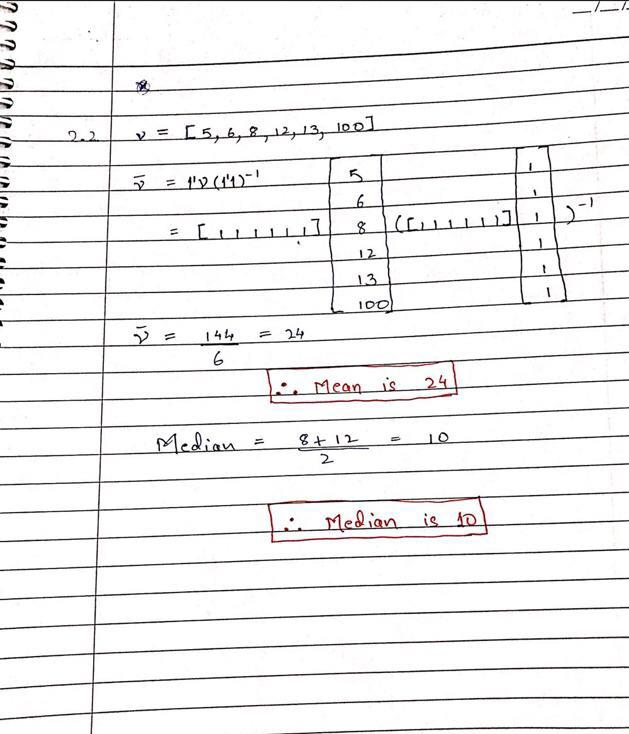
\includegraphics[scale=0.5]{resources/vector.jpeg}
    \caption{Solution}  
    \label{fig:Solution}
\end{figure}
    \end{enumerate}
    
    \item Given the following hypothesis say whether they are falsifiable, and explain why.
        \begin{itemize}
            \item \emph{All swans are white.}
            \begin{enumerate}
            \item This hypothesis is falsifiable.
            \item We can falsify the above hypothesis by finding a swan which is not white.
            \end{enumerate}
            \item \emph{She will go running, when it rains or not.}
            \begin{enumerate}
            \item The above hypothesis is falsifiable.
            \item We can falsify the above hypothesis by finding an instance where she doesn't go running, when it rains or not.(Maybe a day when she is sick and is unable to go running)
            \end{enumerate}
            \item \emph{The grass is wet, so it must have rained.}
            \begin{enumerate}
            \item The above hypothesis is falsifiable.
            \item We can falsify the above hypothesis by finding an occasion when it doesn't rain but the grass is still wet (maybe the grass is wet due to water from sprinkler).
            \end{enumerate}
        \end{itemize}
    \item Given the plot in Figure \ref{fig:log_plot}\footnote{Based on       \url{https://en.wikipedia.org/wiki/File:Internet\_Hosts\_Count\_log.svg} }  formulate \textbf{one} sentence that describes the plot.
    \begin{enumerate}
    	\item There is significant rise in the number of internet hosts with less than 10 internet hosts in the year 1970 to over 1G hosts by 2018.
    \end{enumerate}
\end{enumerate}

\begin{figure}[h]
    \centering
    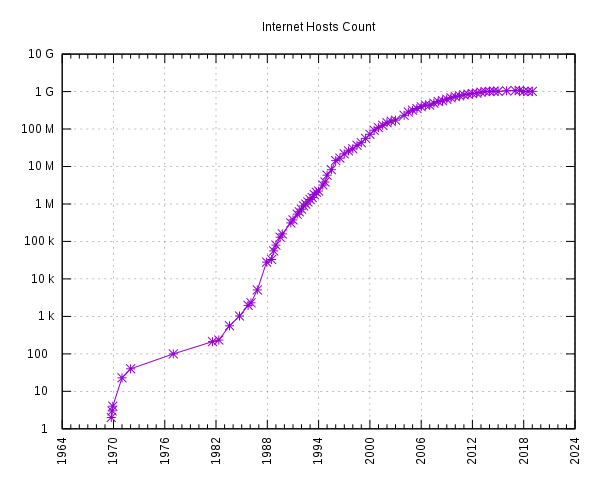
\includegraphics[scale=0.5]{resources/Internet_Hosts_Count_log.png}
    \caption{Number of Internet Hosts Counts}  
    \label{fig:log_plot}
\end{figure}
\end{document}